\documentclass[english, a4paper, oneside, onecolumn, openany,article]{memoir}
\usepackage{fix-cm,fixltx2e}
\usepackage{babel}  % babel: Hyphenation patterns and language specific strings
\usepackage{varioref}
\usepackage[colorlinks,linkcolor=black,urlcolor=black,citecolor=black]{hyperref}
\usepackage[colorinlistoftodos]{todonotes}
\usepackage[latin1]{inputenc}
\usepackage{graphicx}
\usepackage{listings}
\usepackage[square,numbers]{natbib}
\usepackage{url}
\usepackage{pslatex}
\usepackage{multirow}
\usepackage[T1]{fontenc}
\usepackage{eso-pic}
\usepackage{xcolor,calc}
\usepackage{pdfpages}
\newsubfloat{figure}
\usepackage{placeins} % gives me FloatBarrier
%Forhindrer floats i at flyde ind i næste afsnit
\let\oldsection=\section % gemmer den gamle definition
\renewcommand\section{\FloatBarrier\oldsection}

\makeatletter
\renewcommand\fps@figure{htbp} % Force figure placement
\renewcommand\fps@table{htbp}
\makeatother

% setup captions
\hangcaption
\changecaptionwidth
\captionwidth{9cm}


\title{Advanced Data Management - Assignment 2}
\author{S\o ren Bjerregaard Vrist - 151082-sbvr@itu.dk\\ \\Undervisere: Philippe
Bonnet - phbo@itu.dk og
Rasmus Pagh - pagh@itu.dk\\ITU Copenhagen}


\begin{document}
\maketitle
\newpage
\chapter{Part1 - Writes}
\section{Part1a}
The objective is to try to experiment with write performance of DB2. 
First the baseline performance of an EC2 small instance running Ubuntu 9.10 with
``out-of-the-box'' db2 is reported. After that I've tried different tuning knobs
to in someway affect the insert performance.

Overall was it hard to find basis for experimentation. What can be improved and
how? 

\subsection{Results}
All experiements has been done via a comprehensive list of bash scripts included
in the appendix. The ``setup.bash''(Appendix \ref{app:setup} script contains all the auxiliary
information needed when running the experiments, including snapshot and vmstat
output. As descriped in the log (Section \ref{log:probwrite}) the writes.py had
problems so I decided to use my own edition of writes.py \footnote{profwrites2.py -
Appendix \ref{app:prof}} for all the following experiments.


\subsubsection{Baseline}
The baseline (for me) is the defaults from writes.py (5 runs, 10 threads,
InsertN,$100.000$ writes, 1.000.000 tuples). 
\begin{itemize}
  \item 17.1 seconds.
\end{itemize}
Vmstat doesnt show that it is IO bound:
\begin{verbatim}
procs -----------memory---------- ---swap-- -----io---- -system-- ----cpu----
 r  b   swpd   free   buff  cache   si   so    bi    bo   in   cs us sy id wa
...
 1  0      0 107032   4232 1315788    0    0     0    28   63   32 38  0  0  0
 9  1      0  63144   4276 1317044    0    0   300    48  110  299 29  7  1  3
12  1      0  57296   4296 1318260    0    0    62   818  116 10326 30  9  0  0
12  1      0  57296   4304 1318260    0    0     0  1210  117 14254 30  8  0  0
 9  0      0  57296   4328 1318260    0    0     4  1070  103 13700 30  8  0  0
12  1      0  57296   4328 1318260    0    0     0  1136   96 14041 31  7  0  0
 7  0      0  56232   4340 1319292    0    0     2  1066  120 13615 30  9  1  0
10  1      0  53192   4348 1322356    0    0     0  1050  107 13204 30  8  0  0
11  1      0  49544   4360 1325940    0    0     2  1008  103 13377 28 10  0  0
 3  0      0  69824   4360 1325912    0    0    24   638   90 8580 25 13  0  0
10  1      0  49080   4376 1325976    0    0     0   398   81 5465 31  7  0  0
11  1      0  48320   4380 1325992    0    0     2   900  112 11977 27 11  0  0
13  1      0  47000   4384 1326048    0    0    26   950  111 12514 26 12  0  0
11  1      0  44116   4392 1316488    0    0   510  1012  138 12102 26 12  0  0
 2  1      0  49896   4428 1300924    0    0    10   960  117 11966 26 11  0  0
 7  1      0  44416   4436 1302568    0    0   115   982  115 12887 29  9  0  0
14  1      0  41832   4444 1293864    0    0     0   910  105 11997 25 12  0  0
 9  1      0  44712   4328 1289512    0    0    68   844  107 11655 30  8  0  0
...
\end{verbatim}
Around 1000 in the ``bo'' column. Block/s sent to device). 
When measuring disk performance 20-60.000 is possible.

\subsubsection{Threads}
Maybe concurrency could improve this?
(I expected that it would actually be best with as few threads as possible
because of the RR isolation level). Figure \ref{fig:part1athreads}\footnote{This
experiment was rerun after the AUTO\_COMMIT bug was found} confirms my
suspicion that fewer threads are beneficial (due to locking when RR insolation
level is used).
\begin{figure}
  \centering
  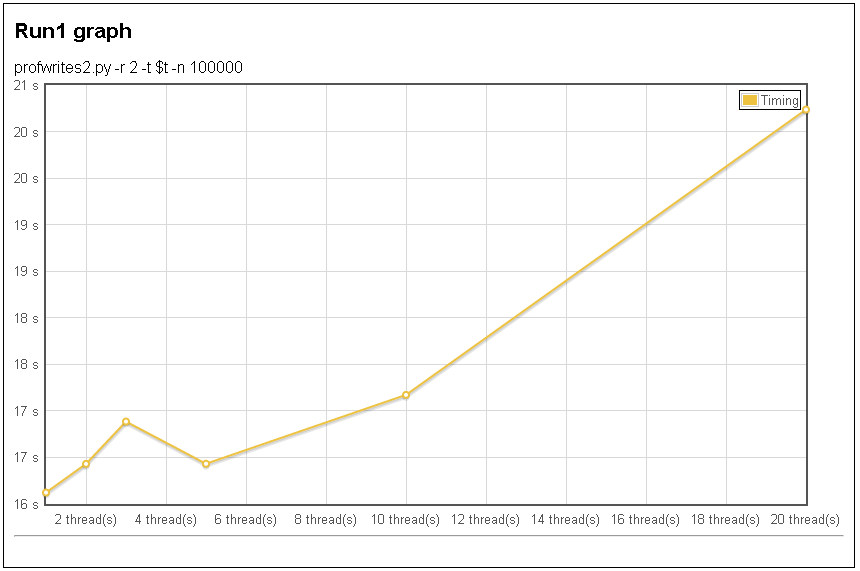
\includegraphics[width=12cm]{assignment2/run1}
  \caption[Insert performance]{Graph of insert timing for 100.000 rows(in one
  transaction) as a function of concurrency}\label{fig:part1athreads}
\end{figure}

\subsubsection{Indexes/primary key on table}
My next theory was that it might be because the time was spent maintaining index
integrity while inserting. The timing results can be seen in figure
\ref{fig:part1aindex1}. Concurrency still gives a penalty, but it is a couple of
seconds faster for all concurrency level without a private key (and thereby an
index).
\begin{figure}
  \centering
  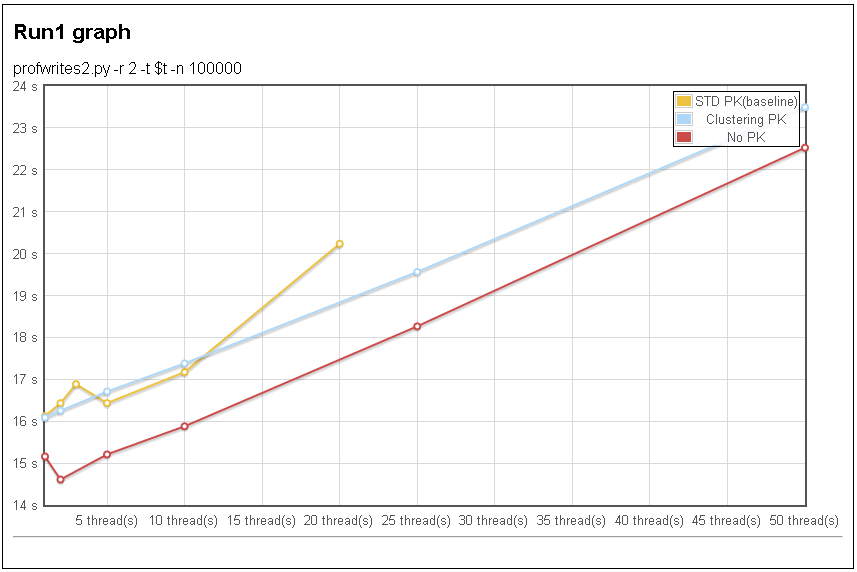
\includegraphics[width=12cm]{assignment2/run1index}
  \caption[Insert performance]{Graph of insert timing for 100.000 rows(in one
  transaction -x1) as a function of concurrency - differnt kinds of indexes}\label{fig:part1aindex1}
\end{figure}

To support this, this unified diff of DB2 snapshot information illustrates
the difference:
\begin{verbatim}
-Buffer pool index logical reads            = 574013
-Buffer pool index physical reads           = 27
+Buffer pool index logical reads            = 48
+Buffer pool index physical reads           = 23
\end{verbatim}
``-'' prefixes with normal primary key and ``+'' prefixes the snapshot when
inserting into a table without primary key (and thereby without index).

Additionally this can also be seen in the log activity:
\begin{verbatim}
-Log pages written                          = 7708
-Log write time (sec.ns)                    = 23.000000004
-Number write log IOs                       = 1137
+Log pages written                          = 3364
+Log write time (sec.ns)                    = 18.000000004
+Number write log IOs                       = 865
\end{verbatim}

This only means that I've minimized the time spent doing ``superflous''
activity. When loggin at vmstat output, this actually means the we see even less
write activity to the disk with a possibility of writing somewhere around
100times as much data per second before we hit a disk bottleneck.

My best guess in this situation is that the time then is spent doing
housekeeping around table structures. DB2 contains a feature to set a table into
``append mode'' somewhat similar to remove indexes from the table. Maybe
additional performance can be found here?
\begin{figure}
  \centering
  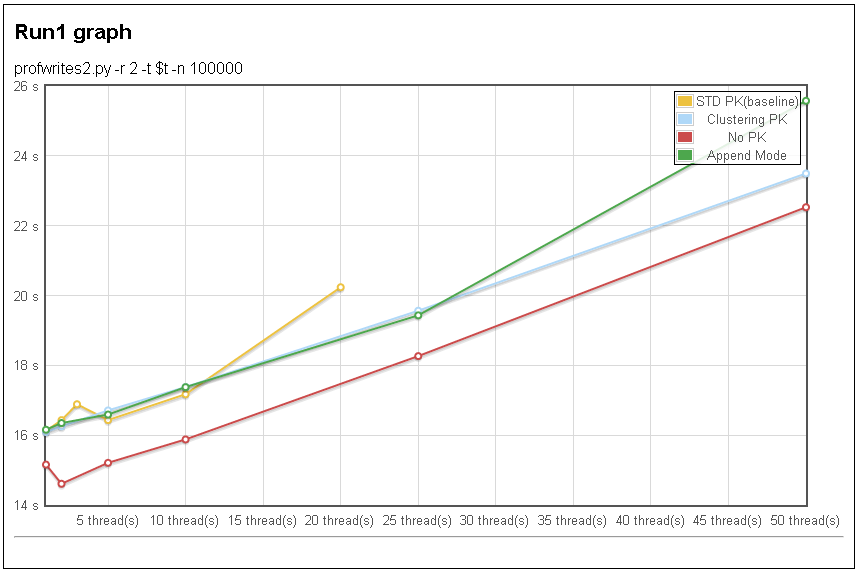
\includegraphics[width=13cm]{assignment2/run1append}
  \caption[Insert performance]{Graph of insert timing for 100.000 rows(in one
  transaction -x1) as a function of concurrency - incl append mode}\label{fig:part1aappnd}
\end{figure}

Figure \ref{fig:part1aappnd} added another line to the graph from figure
\ref{fig:part1aindex1}. No improvement what so ever.

\subsubsection{Log knobs}
Then maybe some database parameters will allow me to speed up insertion rate. I
chose the size of the Log Buffer (LOGBUFSZ) and the Changed Page Threshold.
Firstly a larger log buffer(or disabling it) will prolong the time between log
buffer flushes (or remove them completely).
\begin{figure}
  \centering
  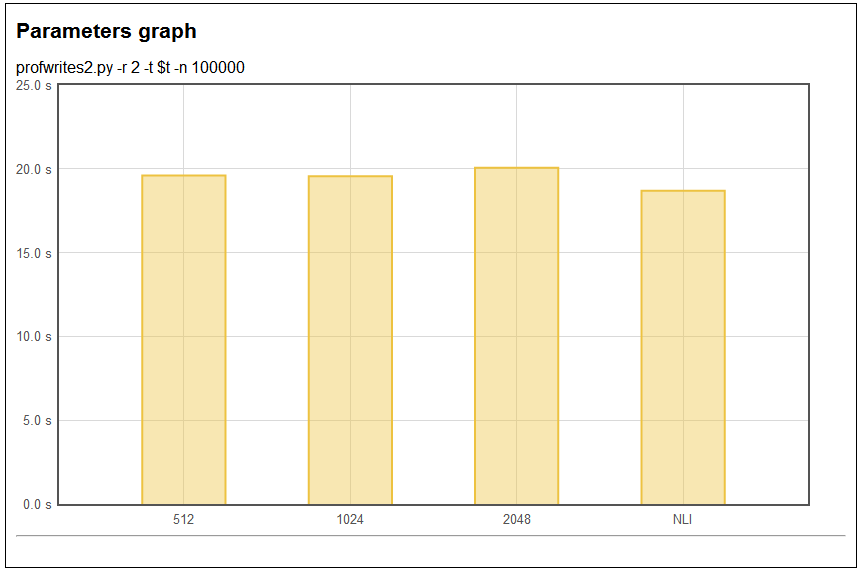
\includegraphics[width=12cm]{assignment2/logb}
  \caption[Insert performance -logbufsz]{Graph of insert timing for 100.000 rows(in one
  transaction -x1) with different LOGBUFSZ (and disabled)}\label{fig:part1alogb}
\end{figure}
Figure \ref{fig:part1alogb} shows no remarkable improvement with different
LOGBUFSZ parameters. Only disabling log altogether gives a small improvement. By
disabling the log all recovery is impossible and is in my oppinion a
``dangerous'' choice for performance.

CHNGPGS\_THRESH decides when the buffer pool writes dirty pages to disk
 asynchronously. With low values pages are ``agressively'' written to disk and
 higher values postpones the effort.
\begin{figure}
  \centering
  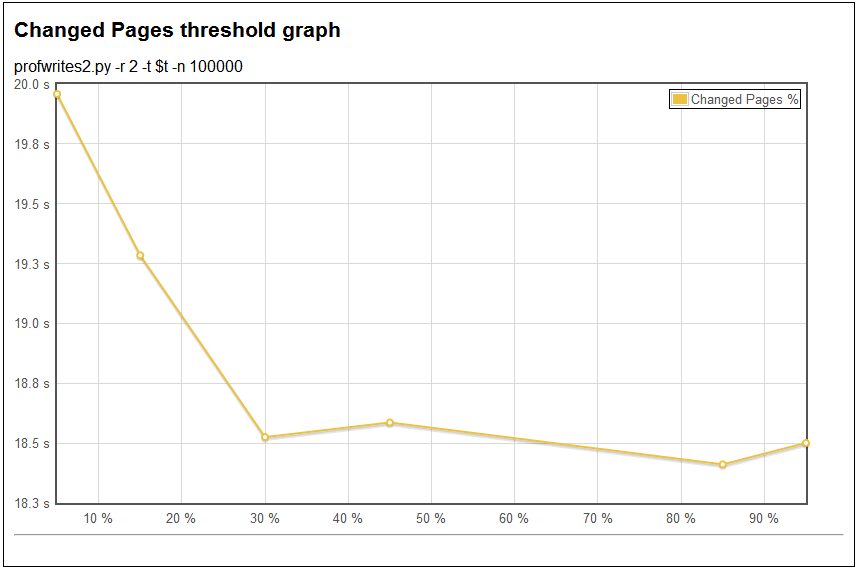
\includegraphics[width=12cm]{assignment2/chpgs}
  \caption[Insert performance - chgpgs]{Graph of insert timing for 100.000 rows(in one
  transaction -x1) with different CHNGPGS\_THRES}\label{fig:part1achgs}
\end{figure}
In figure \ref{fig:part1achgs} we see that as long as chgpgs is larger than 30\%
the performance is unaffected.
\subsection{Conclusion}
I had all in all a very hard time to push DB2 to use more disk I/O (and thereby
being faster). Only the indexes could give a couple of seconds improvement.

\section{Part1b}
The objective is to see if tablelocking can improve insert/updater performance.
\subsection{Results}
Due to particulars around table locking these experiments was run with 1 run on
1 thread. As figure \ref{fig:part1btl} shows, no improvement was seen with
tablelocking. \footnote{I reran this experiment after the AUTO\_COMMIT bug, but
still nothing}.

\begin{figure}
  \centering
  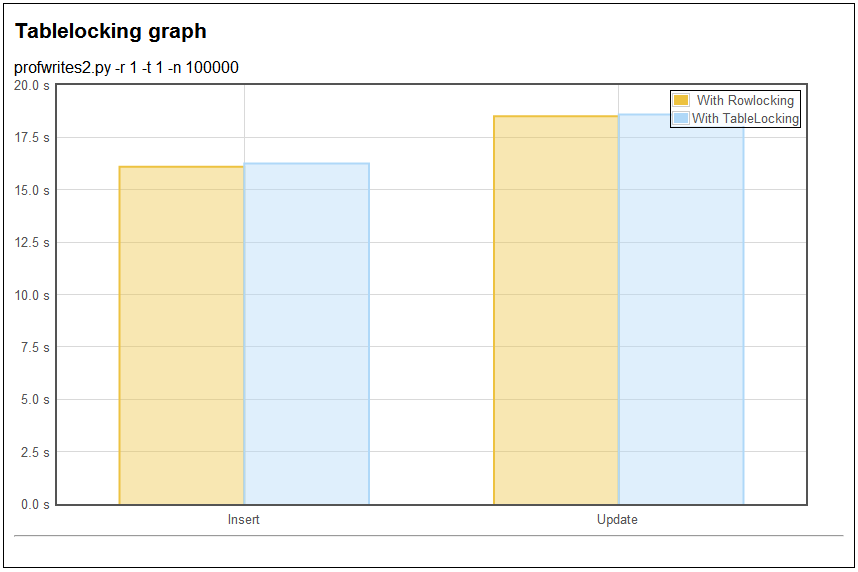
\includegraphics[width=12cm]{assignment2/tl}
  \caption[Insert/update performance -Table locking]{Graph of insert/update timing for 100.000 rows(in one
  transaction -x1) with/without tablelocking}\label{fig:part1btl}
\end{figure}

\chapter{Part2 - Reads}

\section{Part2a}
The first investigations showed some inconsistencies in the runtime over a
complete table scan. See the log book in Section \ref{logb:part2}, and this
experiment I used db2batch instead.

I tried tuning the BufferPool size, prefetching, LogBufferSize and indexes as
graphed in Figure \ref{fig:readio}.

\begin{figure}
  \centering
  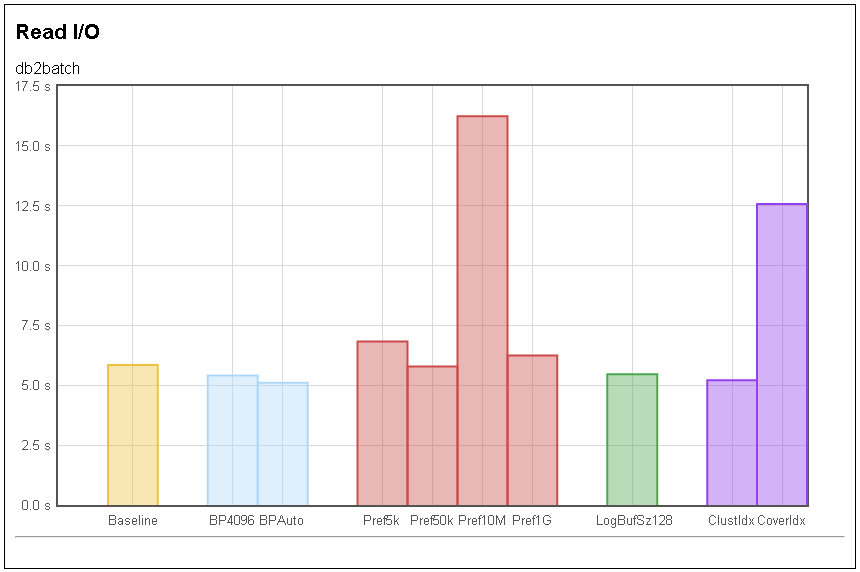
\includegraphics[width=12cm]{assignment2/readio}
  \caption[Read performance - Table locking]{Graph of read timing for 2.500.000
  rows with different parameters tweaked}\label{fig:readio}
\end{figure}

Figure \ref{fig:readio} shows that none of my tweakings gave any better
performance. Prefetching set to 10Mb was clearly not a good idea as well as a
covering index gave additional overhead. I have no good explanation for the
overhead associated with a prefetch of 10Mb. The snapshot statistics shows that
the buffer might have been flushed due to the prefetch side which leads to many
physical reads from the bufferpool:
\begin{verbatim}
Baseline   : Buffer pool data physical reads = 102
Prefetch10M: Buffer pool data physical reads = 28242
\end{verbatim}
The covering index is slower since the query planner decides to use the index
adding an additional layer of datastructures eventhough no sorting is needed and
the complete table will be scanned any way:\\
\noindent\begin{tabular}{p{5cm}|p{5cm}}
  Covering Index & No index
 \\
\begin{verbatim}
Optimizer Plan:

    Rows   
  Operator 
    (ID)   
    Cost   
          
  2.5e+06 
    n/a   
  RETURN  
   ( 1)   
  24532.6 
    |     
  2.5e+06 
    n/a   
  IXSCAN  
   ( 2)   
  24532.6 
    |     
 2.5e+06  
 Index:   
 DB2INST1 
 NC3      
\end{verbatim}
&
\begin{verbatim}
Optimizer Plan:

    Rows   
  Operator 
    (ID)   
    Cost   
          
  2.5e+06 
    n/a   
  RETURN  
   ( 1)   
  31354.9 
    |     
  2.5e+06 
    n/a   
  TBSCAN  
   ( 2)   
  31354.9 
    |      
  2.5e+06  
    n/a    
 Table:    
 DB2INST1  
 EMPLOYEES 
\end{verbatim}
\\
\hline
\end{tabular}

\section{Part2b - Clustering index}
Multipoint query which should show that an index can help with performance, and
show the difference between a clustering and normal index. My graph in Figure
\ref{fig:clust} shows the same order of magnitude improvement in throughput when
using and index. The difference between clustered and non clustered index is a
best minimal if not opposite to the graph from the book.
\begin{figure}
  \centering
  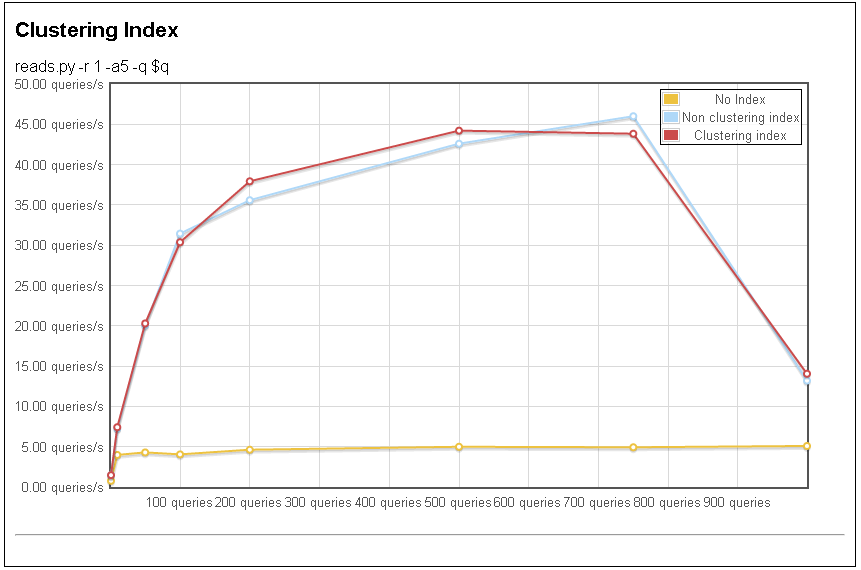
\includegraphics[width=12cm]{assignment2/clust}
  \caption[Read performance - Clustering Index]{Graph of read timing as a
  function of multi\_point queries for different index types. }\label{fig:clust}
\end{figure}

The index provides an efficent (b-tree+) way to do lookup for a given value in
the table. Without an index all rows must be scanned to find matches which
explains the difference between using an index and not. A clustering index
orders the data in the table based on the index columns such that ``close
values'' are close in the table. This should provide an additional benefit when
doing multipoint queries as all results matching a criteria will be close and
additional lookup be limited. This is not quite obvious in my experiment, which
might be due to the non-clustering index implictly doing clustering or similar
optimization techniques.

\section{Part2c - Covering index}
This experiment should investigate how a covering index - that is an index
containing all columns being used in both where clause and select clause -
compares to lesser indexes and a clustering indexes as well as the ordering of
the columns in the index definition.
\begin{figure}
  \centering
  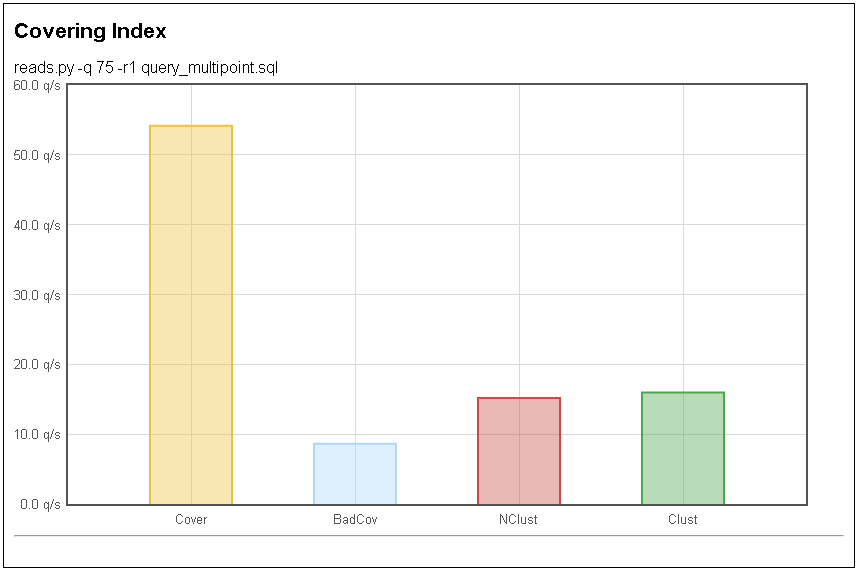
\includegraphics[width=12cm]{assignment2/cover}
  \caption[Read performance - Covering Index]{Graph of read throughput comparing a
  covering index to other index types}\label{fig:cover}
\end{figure}
Figure \ref{fig:cover} shows the result of my experiment. As in the book a good
covering index (the equality columns first, then the select columns) is the best
choice where as a bad covering index actually is slower than a non covering
index.

\section{Part2d - Selectivity}
As seen in the part1a using an index for selecting many rows can give additional
overhead. This experiement compares the performance of selecting increasing
percentage of the table contents between an index and using no index.\\

As noted in the log book(Section \ref{logb:part2}) the reads.py didnt actually
fetch the rows found by the query, so to get reasoable results for this
experiment I had to add some additional code to reads.py.

\begin{figure}
  \centering
  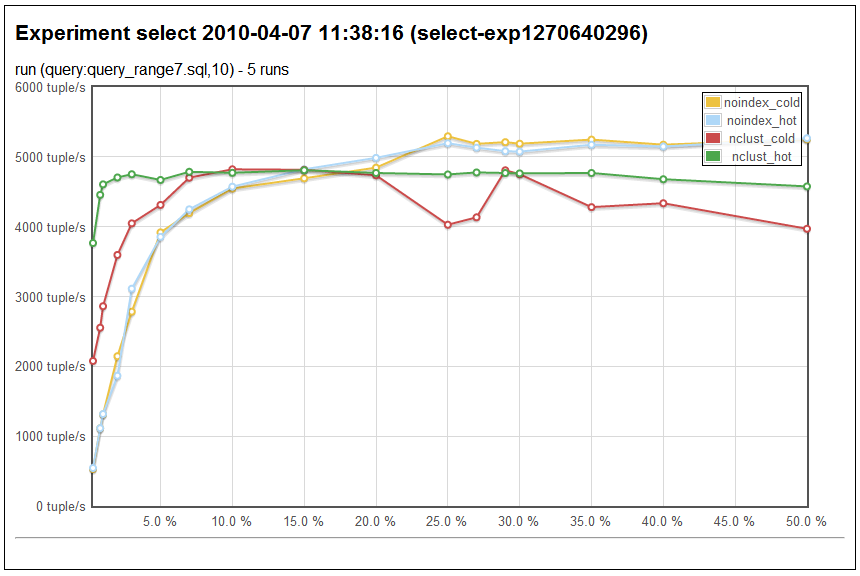
\includegraphics[width=12cm]{assignment2/select}
  \caption[Read performance - Index vs. Scan]{Graph of throughput as a function
  of percentage of a complete table selected for both a non-clustering index and
  with out}\label{fig:select}
\end{figure}

Figure \ref{fig:select} shows that an index is the best choice up until when
15\% or more is returned by the query. After that it is more efficent to scan
the complete table.


\chapter{Log book over experiments}

\section{Part 1}

\subsection{Problems with writes.py}\label{log:probwrite}
\begin{itemize}
  \item[2010-03 16-20] Noticed no IO when executing run 2..n of part1a.
    \begin{itemize}
      \item Changed writes.py to use multiprocessing.Pool and allow for writes on
    all runs (Appendix \ref{app:prof}) as well as remove the shared mutex
    between threads there by removing a heavy bottleneck on system level Context
    switches.
   \end{itemize}
  \item Executed 10runs to flatten out any outlieres with amazon ec2 with each
    (Appendix \ref{app:setup})
  \item[2010-03 21] Part1b in the assignement text says that you need to use a \verb|db2 +c|\ldots
    command to enforce a tablelock. That doesnt work because the script uses
    another connection. Changed the script to contain a ``lock table'' part.
    (Included in appendix \ref{app:tl} and was also added to my profwrites2.py
    script).
  \item[2010-04 04] Read newsgroup and read that a bug existed in writes.py
    concerns the ``AUTO\_COMMIT'' parts of the code.\\
    Fixed the script and verified that my old experiments is void:
    \begin{itemize}
      \item Run from 2010-03-20: \verb|Commit statements attempted  = 500037|
      \item Run from 2010-04-04 with fixed script \verb|Commit statements attempted  = 4|
    \end{itemize}
    Notice that the scripts included in the appendix ARE fixed now. 
    This affects all experiments until today, including assignment1.
\end{itemize}

\section{Part2}\label{logb:part2}
\begin{itemize}
  \item[2010-04-01:] My investigations show that reads.py  doesnt actually fetch
    the rows, even though ibm\_db.execute executes a query that encompass the
    complete table. Both vmstat and the run time suggest this. I decided to use
    db2batch for at least part2a.
  \item[2010-04-07:] Needed a usable reads.py for part2d. Added this to force
    reads.py to actually do the IO:
\begin{verbatim}
rowcount=0
dict = ibm_db.fetch_assoc(query_stmt)
while dict != False:
   rowcount +=1
   dict = ibm_db.fetch_assoc(query_stmt)
print ``rc: %d''%(rowcount) 
\end{verbatim}
The print part is not important, but ``fetch\_assoc'' (or one of the other
fetch\_) is needed.
   \item[2010-04-07:] Needed a way to fast graphing part2d experiments.
     Developed yet another script for parsing experiment output and generate
     flot js files. Included in appendix \ref{app:parseexperiment}
\end{itemize}

\appendix
\newpage
\chapter{Appendix}
\section{Profwrites2.py}\label{app:prof}
New edition of the writes.py that does work on subsequent runs as well as no
shared mutex.
\lstinputlisting{assignment2/profwrites2.py}

\section{Parse\_experimnet.py}\label{app:parseexperiment}
\lstinputlisting{assignment2/parse_experiment.py}


\section{writestl.py}\label{app:tl}
New edition of the writes.py that contains a tablelocking switch.
\lstinputlisting{assignment2/writestl.py}

\section{setup.bash and experiment execution}\label{app:setup}
To even out any ec2 glitches I ran the experiements several times:
\begin{verbatim}
$ for i in `seq 3`; 
do 
   echo $i; 
   bash run1.bash; 
   bash run2.bash; 
   bash tl.bash; 
done
\end{verbatim}

\subsection{Tool script included by all experiment specific scripts}
\lstinputlisting{assignment2/setup.bash}

\subsection{Experiment scripts for assignment2-part1}

Part1a:\\
Different threadcounts and index/private key/append mode for tables.
\lstinputlisting{assignment2/run1.bash}
Part1a:\\
Experiment with LOGBUFSZ, CHNGPGS\_THRES values.
\lstinputlisting{assignment2/run2.bash}
Part1b:\\
Tablelocking both insert and updates.
\lstinputlisting{assignment2/tl.bash}
\subsection{Experiment scripts for assignment2-part2}
Part2a:\\
\lstinputlisting{assignment2/logb.bash}

Part2b:\\
\lstinputlisting{assignment2/clust.bash}

Part2c:\\
\lstinputlisting{assignment2/cover.bash}

Part2d:\\
\lstinputlisting{assignment2/select2.bash}

\end{document}
